\chapter{Dataset and Data Understanding}
\label{chap:datasets-setup}
\setlength{\emergencystretch}{1.5em}

This chapter describes the dataset used to drive the simulator and the
exploratory analysis performed prior to policy training.  It documents the
source and structure of the ITU/Zindi telecom energy dataset, the
preprocessing steps used to prepare site-level time series, and the
cross-site heterogeneity that motivates multi-site evaluation.

The exploratory data analysis (EDA) presented in this chapter serves two
purposes: (i) to characterise the operational variability across telecom
sites in terms of load demand, solar generation, and grid availability, and
(ii) to identify the structural conditions that motivate the
inventory-aware control problem studied in this thesis.  In particular,
the analysis highlights the temporal mismatch between load and solar
generation, the heterogeneity in outage patterns across sites, and the
resulting reliability stress that motivates explicit diesel inventory
management.

The purpose of this chapter is not to redefine the control problem, which
was formalised in Chapter~\ref{chap:problem}, but to show how the exogenous
signals used by the implemented environment arise from the data and why
they make the problem non-trivial.


% ============================================================
\section{Dataset Overview}
\label{sec:dataset_overview}
% ============================================================

The experimental study uses the ITU 2024 Smart Energy Scheduling Challenge
dataset released through the Zindi platform~\citep{itu2024zindi}.  The
processed dataset contains ten independent telecom tower sites, each observed
for 60 days at hourly resolution ($\Delta t = 1$\,h), yielding 1{,}440 rows
per site and 14{,}400 rows in total.  The same dataset has been used in
recent telecom energy scheduling work, making it a suitable benchmark for
comparison-oriented research.

\begin{table}[htb]
\centering
\small
\caption{Processed dataset summary.}
\label{tab:dataset_overview}
\begin{tabular}{ll}
\toprule
\textbf{Property} & \textbf{Value} \\
\midrule
Source              & ITU 2024 Smart Energy Scheduling Challenge (Zindi) \\
Sites               & 10 telecom tower sites \\
Duration            & 60 days per site \\
Temporal resolution & Hourly ($\Delta t = 1$\,h) \\
Rows per site       & 1{,}440 \\
Total rows          & 14{,}400 \\
Processed format    & One CSV per site + merged master time series \\
Validation          & All 10 sites pass schema and range checks \\
\bottomrule
\end{tabular}
\end{table}

Each processed site file contains the variables listed in
Table~\ref{tab:variables}.  These correspond directly to the exogenous
components of the CMDP introduced in Chapter~\ref{chap:problem}.

\begin{table}[htb]
\centering
\small
\caption{Processed dataset variables and their role in the simulator.}
\label{tab:variables}
\begin{tabular}{lllp{5.2cm}}
\toprule
\textbf{Column} & \textbf{Symbol} & \textbf{Units} & \textbf{Role} \\
\midrule
\texttt{load\_kwh}              & $P_t^{\Load}$ & kWh/h   & Tower load demand (exogenous) \\
\texttt{solar\_kwh}             & $P_t^{\PV}$   & kWh/h   & Solar generation (exogenous) \\
\texttt{grid\_available}        & $G_t$         & Boolean & Grid availability indicator \\
\texttt{net\_load\_kwh}         & $P_t^{\Net}$  & kWh/h   & Derived: load minus solar \\
\texttt{battery\_capacity\_kwh} & $E_{\Bat}$ & kWh & Site battery capacity (constant per site) \\
\texttt{dg\_power\_kw}          & $P^{\DG}_{\rated}$ & kW & DG rated output (site parameter, constant) \\
\texttt{grid\_power\_kw}        & $P^{\Grid}_{\max}$ & kW & Maximum grid draw (site parameter, constant) \\
\texttt{t}, \texttt{day}, \texttt{hour} & ---   & index   & Time indexing for rollouts \\
\bottomrule
\end{tabular}
\end{table}

The dataset does not include diesel delivery logs, in-transit fuel records, or
replenishment events.  Consequently, the delivery-pipeline variable $\Pipe_t$
is generated synthetically within the simulator, as described in
Chapter~\ref{chap:methodology}.  All other environment inputs are drawn
directly from the processed site traces.


% ============================================================
\section{Preprocessing Pipeline}
\label{sec:preprocessing}
% ============================================================

Preprocessing is applied identically across all ten sites.

\paragraph{Schema and range validation.}
Each site file is checked for required columns, valid numeric types, and
consistent hourly indexing.  All ten processed site files passed schema and
range checks, and no missing-value imputation was required in the final
processed dataset.

\paragraph{Derived variables.}
Net load is computed as $P_t^{\Net} = P_t^{\Load} - P_t^{\PV}$.  This
quantity separates energy-deficit hours (positive net load) from
solar-surplus hours (negative net load) and is used throughout the EDA
sections below.

\paragraph{Tank capacity derivation.}
Absolute diesel tank capacity is not provided in the dataset.  Tank capacity
is set to $C^{\Tank} = 72\,\bar{D}$ kWh-equivalent, where $\bar{D}$ is the
site mean hourly load, giving approximately three days of full-load backup.
This assumption is applied consistently across all sites and is clearly
labelled wherever capacity is referenced.

\paragraph{Train/test split.}
Each site's 60-day series is split chronologically: days~1--45 form the
training block and days~46--60 the test block.  The split is site-local and
strictly temporal, preventing cross-site or future-to-past leakage.  During
training, episodes start from random hours within the training block;
evaluation is fixed to the 15-day test window with randomised initial
inventory over $[0.3,\,0.9]\,C^{\Tank}$.

\paragraph{Observation normalisation.}
Continuous observations are normalised online using \texttt{VecNormalize}
with Welford's algorithm.  Normalisation statistics are accumulated during
training and frozen before evaluation; the same frozen statistics are applied
to all evaluation rollouts.


% ============================================================
\section{Cross-Site Characteristics}
\label{sec:site_characteristics}
% ============================================================

The ten sites span a broad operating envelope in terms of average load,
solar self-sufficiency, and grid reliability.  This heterogeneity is one of
the main reasons a multi-site evaluation is necessary: a controller that
performs well on a solar-rich, grid-stable site may not generalise to a
high-load, grid-poor site.

Table~\ref{tab:site_stats} provides per-site statistics derived from the
master time series.  Figure~\ref{fig:site_characteristics} plots these along
three dimensions simultaneously.

\begin{table}[htb]
\centering
\small
\caption{Per-site operating statistics (60-day means).}
\label{tab:site_stats}
\begin{tabular}{lrrrrrrl}
\toprule
\textbf{Site} & \textbf{Load} & \textbf{Solar} & \textbf{Solar} & \textbf{Grid} &
\textbf{Bat.\ cap.} & \textbf{DG rating} & \textbf{Class} \\
 & \textbf{(kWh/h)} & \textbf{(kWh/h)} & \textbf{cov.\ (\%)} &
\textbf{avail.\ (\%)} & \textbf{(kWh)} & \textbf{(kW)} & \\
\midrule
site1  & 4.55 & 2.07 &  45.6 & 80.0 & 16.2 & 18.0 & Easy   \\
site2  & 9.66 & 2.47 &  25.6 & 62.2 & 41.0 & 17.6 & Hard   \\
site3  & 5.88 & 3.29 &  56.0 & 67.2 & 41.0 & 12.8 & Medium \\
site4  & 9.56 & 5.28 &  55.3 & 67.8 & 41.0 & 17.6 & Medium \\
site5  & 8.32 & 2.83 &  34.0 & 51.7 & 20.5 & 17.6 & Hard   \\
site6  & 4.24 & 1.78 &  42.0 & 80.0 & 41.0 & 17.6 & Easy   \\
site7  & 4.25 & 2.16 &  50.8 & 62.2 & 20.5 & 18.0 & Medium \\
site8  & 2.14 & 3.24 & 151.6 & 67.2 & 21.6 & 10.8 & Easy   \\
site9  & 4.16 & 2.18 &  52.4 & 67.8 & 21.6 & 12.8 & Medium \\
site10 & 4.08 & 3.27 &  80.1 & 51.7 & 20.5 & 17.6 & Medium \\
\bottomrule
\end{tabular}
\end{table}

\begin{figure}[htbp]
\centering
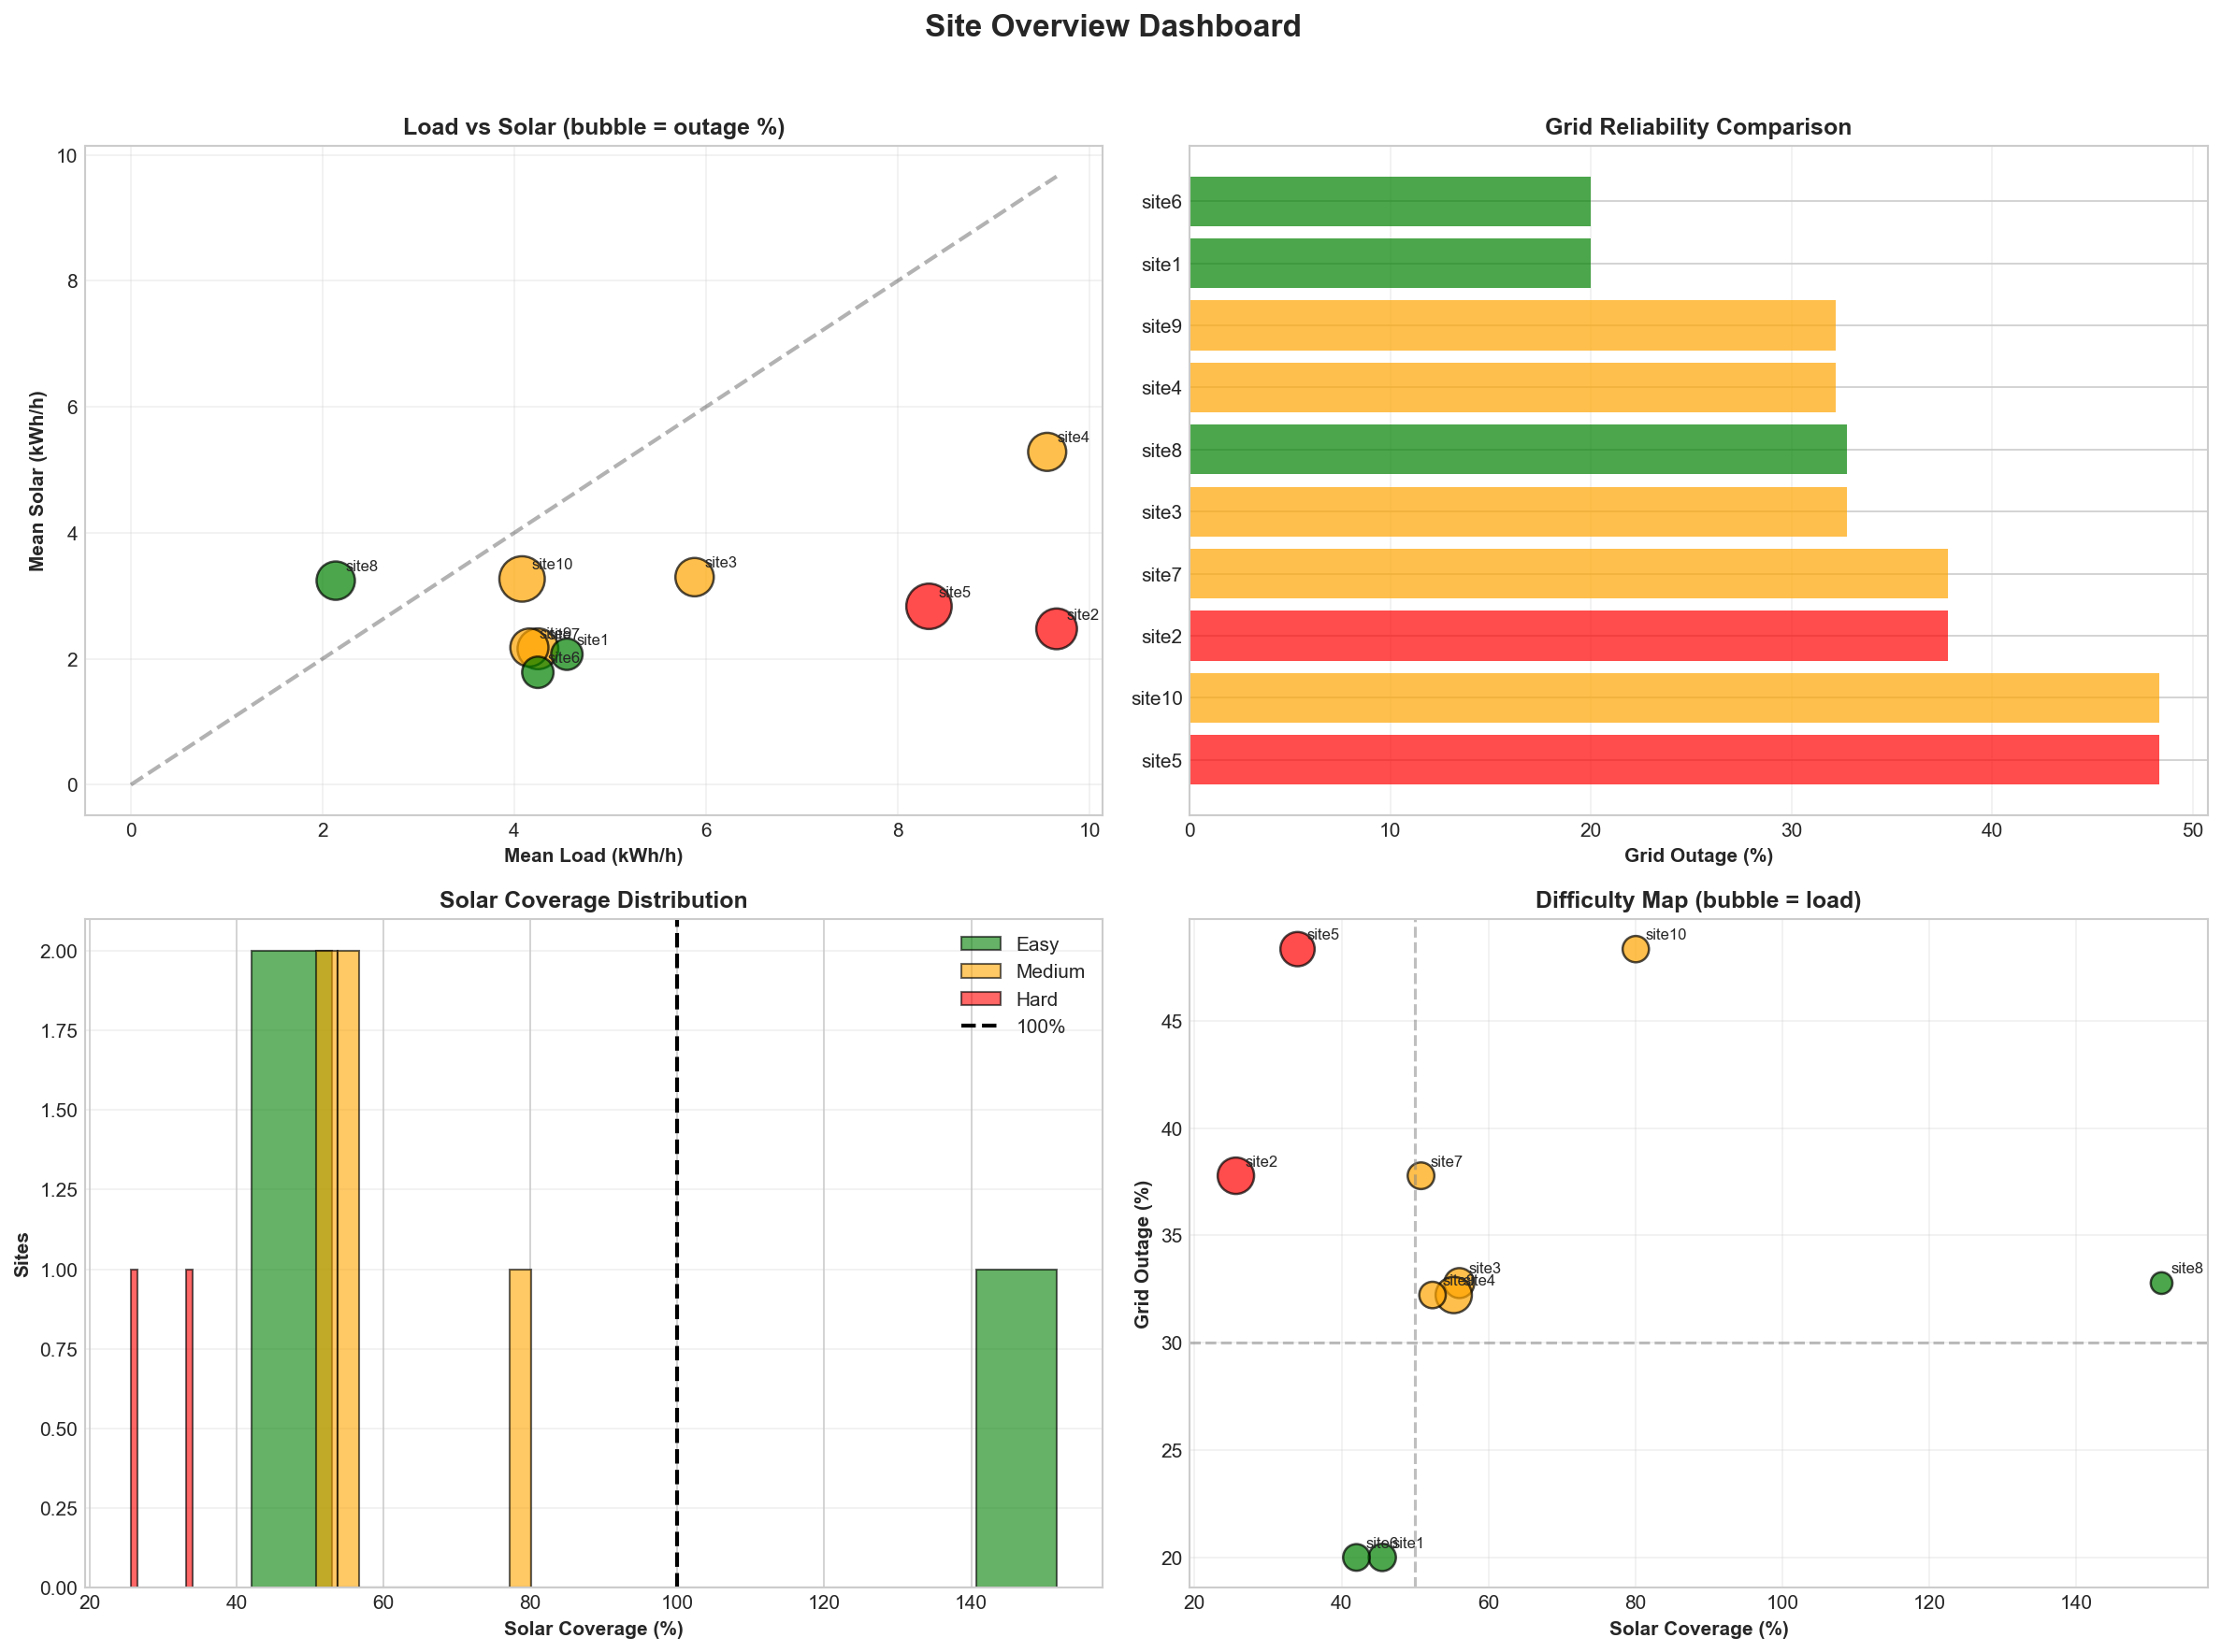
\includegraphics[width=\textwidth, clip=true]{images/fig1_site_overview}
\caption{Site overview dashboard for all ten ITU/Zindi sites.
\textit{Top-left:} mean load vs.\ mean solar scatter; bubble size encodes
outage rate.  Sites above the diagonal are solar-surplus; sites below are
solar-deficit.  \textit{Top-right:} grid outage rate per site, sorted by
severity; sites~5 and~10 have the highest outage exposure ($\approx$48\%).
\textit{Bottom-left:} distribution of solar coverage levels; one site
(site~8) exceeds 100\%.  \textit{Bottom-right:} difficulty map — solar
coverage vs.\ grid outage rate with bubble size proportional to load;
Hard sites (red) occupy the high-outage, low-solar quadrant.}
\label{fig:site_characteristics}
\end{figure}

Three observations emerge from the site statistics.

\textbf{High-load, low-solar, weak-grid sites are the most difficult.}
Sites~2 and~5 combine high average demand (9.66 and 8.32\,kWh/h), poor
solar coverage (25.6\% and 34.0\%), and frequent grid outages (62.2\% and
51.7\% availability).  These sites create persistent energy deficits during
grid loss and place the greatest pressure on diesel backup and fuel inventory
management.

\textbf{Site~8 is solar-surplus.}
With solar coverage of 151.6\%, site~8 generates more PV energy than it
consumes on average.  DG activation is rare; reliability is rarely
threatened.  This site establishes a natural performance ceiling against
which other sites can be compared.

\textbf{Battery capacity is not uniformly matched to load.}
Despite having the highest outage frequency in the dataset, site~5 has only
20.5\,kWh of battery storage --- less than high-load sites~2, 3, and~4 which
carry 41\,kWh banks.  On site~5, diesel inventory is therefore a primary
reliability lever even after battery dispatch is optimised.


% ============================================================
\section{Diurnal Load and Solar Patterns}
\label{sec:diurnal_patterns}
% ============================================================

In addition to cross-site variability, the dataset exhibits a clear and
structured diurnal pattern.  Figure~\ref{fig:diurnal_profiles} shows the mean
hourly load demand and mean hourly solar generation averaged across all sites.

\begin{figure}[htbp]
\centering
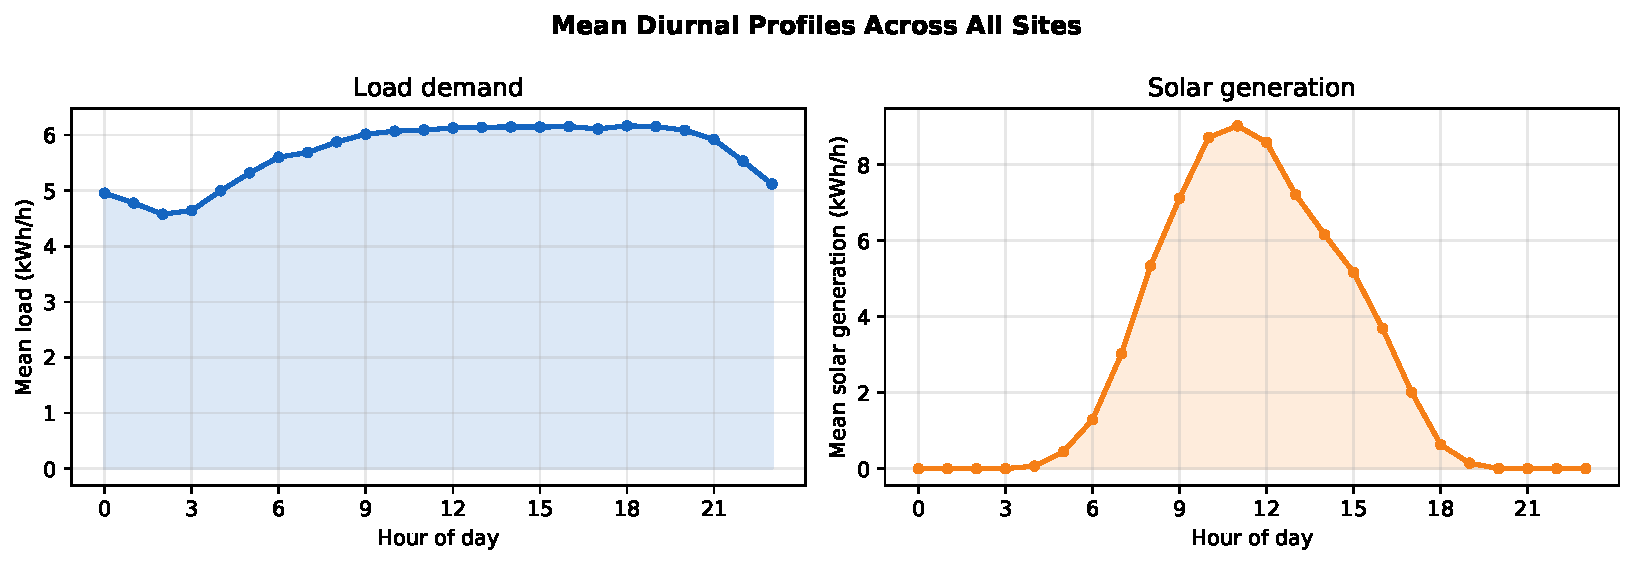
\includegraphics[width=\textwidth, clip=true]{images/fig_diurnal_profiles}
\caption{Mean diurnal load and solar profiles averaged across all ten sites.
Load is elevated from 08:00--20:00, peaking near 6.2\,kWh/h in the
mid-afternoon.  Solar generation peaks near 11:00 at 9.0\,kWh/h before
declining through the afternoon.  The temporal mismatch between peak solar
(11:00) and peak load (14:00--18:00) creates a recurring afternoon deficit
window that battery, grid, or DG must cover.}
\label{fig:diurnal_profiles}
\end{figure}

Two observations are relevant to the control problem.  First, solar generation
is effectively zero from 20:00 to 05:00; all overnight demand must be met by
stored energy, grid supply, or DG operation.  Second, although mean daytime
solar output is substantial, it does not perfectly align with demand: the
solar peak precedes the load peak by several hours.  This creates predictable
deficit windows before sunrise and in the late afternoon, reinforcing the need
for sequential energy management rather than purely myopic dispatch.


% ============================================================
\section{Grid Outage Structure}
\label{sec:grid_patterns}
% ============================================================

Grid availability is a defining feature of the dataset because it is the
primary exogenous disturbance that forces switching between renewables,
battery, and diesel-backed operation.  Figure~\ref{fig:grid_raster} shows the
hour-by-hour outage raster for all ten sites over the full 60-day window.

\begin{figure}[htbp]
\centering
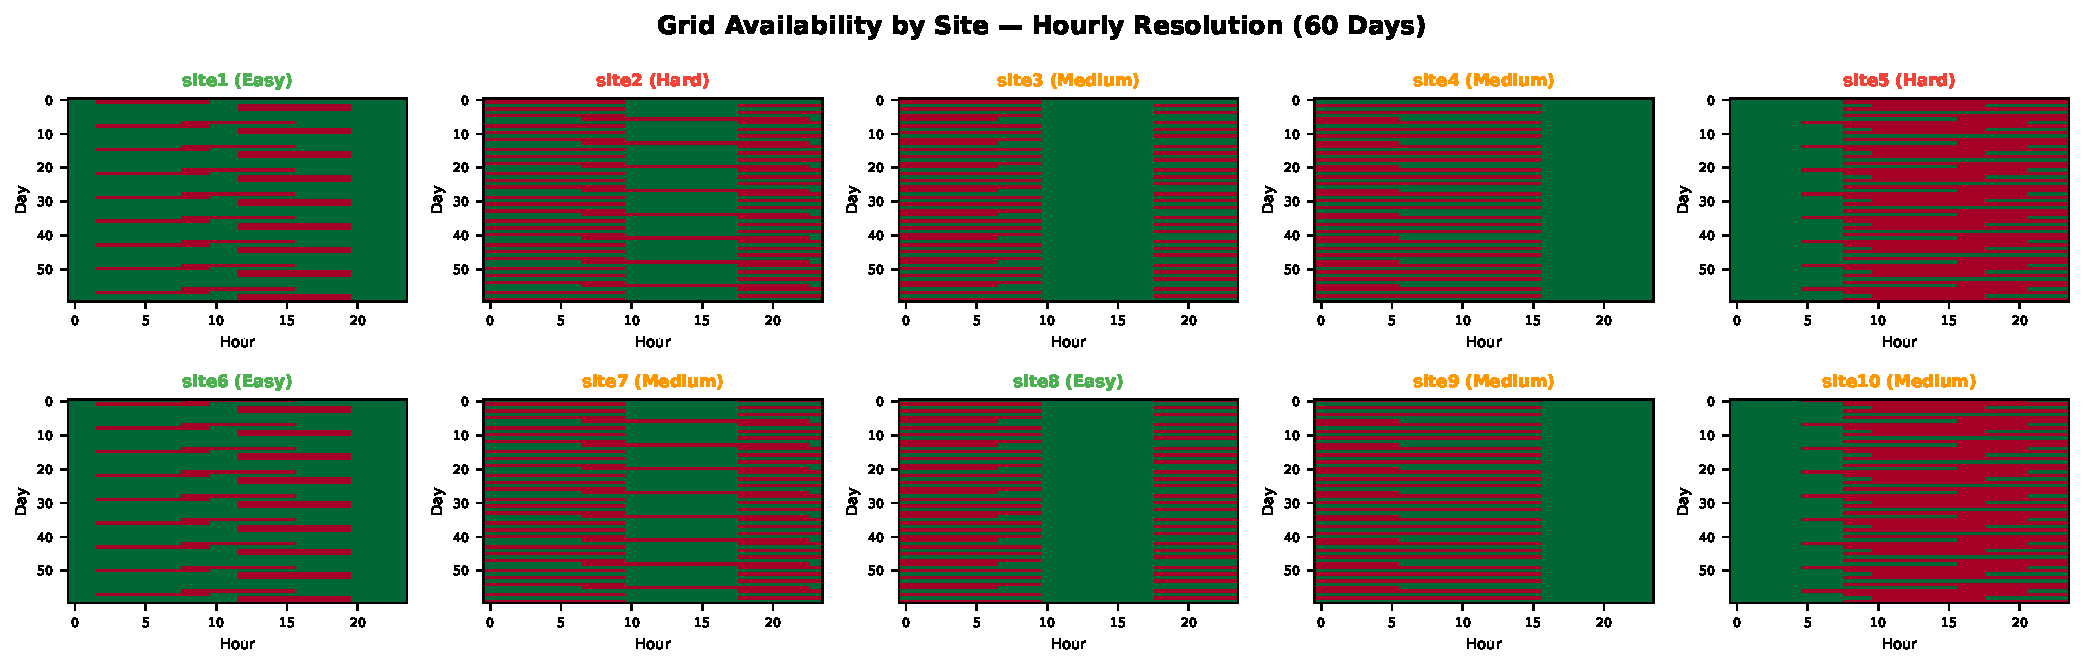
\includegraphics[width=\textwidth, clip=true]{images/fig_grid_raster}
\caption{Grid availability raster: each row is one day, each column one hour
of day.  Green = grid available; red = outage.  Sites~1 and~6 show short,
structured nocturnal outages (8\,h blocks).  Sites~2, 5, 7, and~10 exhibit
extended daily outage patterns (up to 16\,h).  The block structure indicates
that outages are not purely random but follow a predictable daily schedule,
a regularity that a non-myopic RL policy can exploit.}
\label{fig:grid_raster}
\end{figure}

Table~\ref{tab:outage_stats} quantifies outage structure per site.  The
maximum observed outage duration is 16\,h across all sites.  This exceeds the
24-h mean lead time of the normal logistics scenario, confirming that a single
extended outage can deplete a partially-stocked tank before a delivery
arrives --- the core failure mode the inventory-aware policy must prevent.

\begin{table}[htb]
\centering
\small
\caption{Grid outage statistics per site.}
\label{tab:outage_stats}
\begin{tabular}{lrrrl}
\toprule
\textbf{Site} & \textbf{Outage events} & \textbf{Mean duration (h)} &
\textbf{Max duration (h)} & \textbf{Class} \\
\midrule
site1  & 36 &  8.0 &  8 & Easy   \\
site2  & 34 & 16.0 & 16 & Hard   \\
site3  & 34 & 13.9 & 16 & Medium \\
site4  & 34 & 13.6 & 16 & Medium \\
site5  & 52 & 13.4 & 16 & Hard   \\
site6  & 36 &  8.0 &  8 & Easy   \\
site7  & 34 & 16.0 & 16 & Medium \\
site8  & 34 & 13.9 & 16 & Easy   \\
site9  & 34 & 13.6 & 16 & Medium \\
site10 & 52 & 13.4 & 16 & Medium \\
\bottomrule
\end{tabular}
\end{table}

Site~5 stands out with 52 outage events --- the highest frequency in the
dataset --- combined with the lowest solar coverage and a small battery.
This triple constraint makes it the most demanding test for any inventory or
dispatch policy, and it is expected to be among the most informative sites
in the experimental evaluation.


% ============================================================
\section{Scarcity and Surplus Regimes}
\label{sec:scarcity_surplus}
% ============================================================

Exploratory analysis reveals that the dataset naturally separates into two
operational regimes.

\textbf{Scarcity regime.}
In several sites, mean deficit during outage is high and battery autonomy is
insufficient to cover the longest observed outage block.  In such settings,
diesel is not a marginal backup but a critical reliability resource.  A
controller that ignores fuel inventory in these sites risks stockout during
repeated weak-grid periods.  Figure~\ref{fig:rl_stress} quantifies this
across four dimensions: battery autonomy relative to grid outage frequency,
battery sizing against worst-case outage duration, 95th-percentile deficit
severity during outages, and the fraction of solar-surplus hours per site.

\begin{figure}[htbp]
\centering
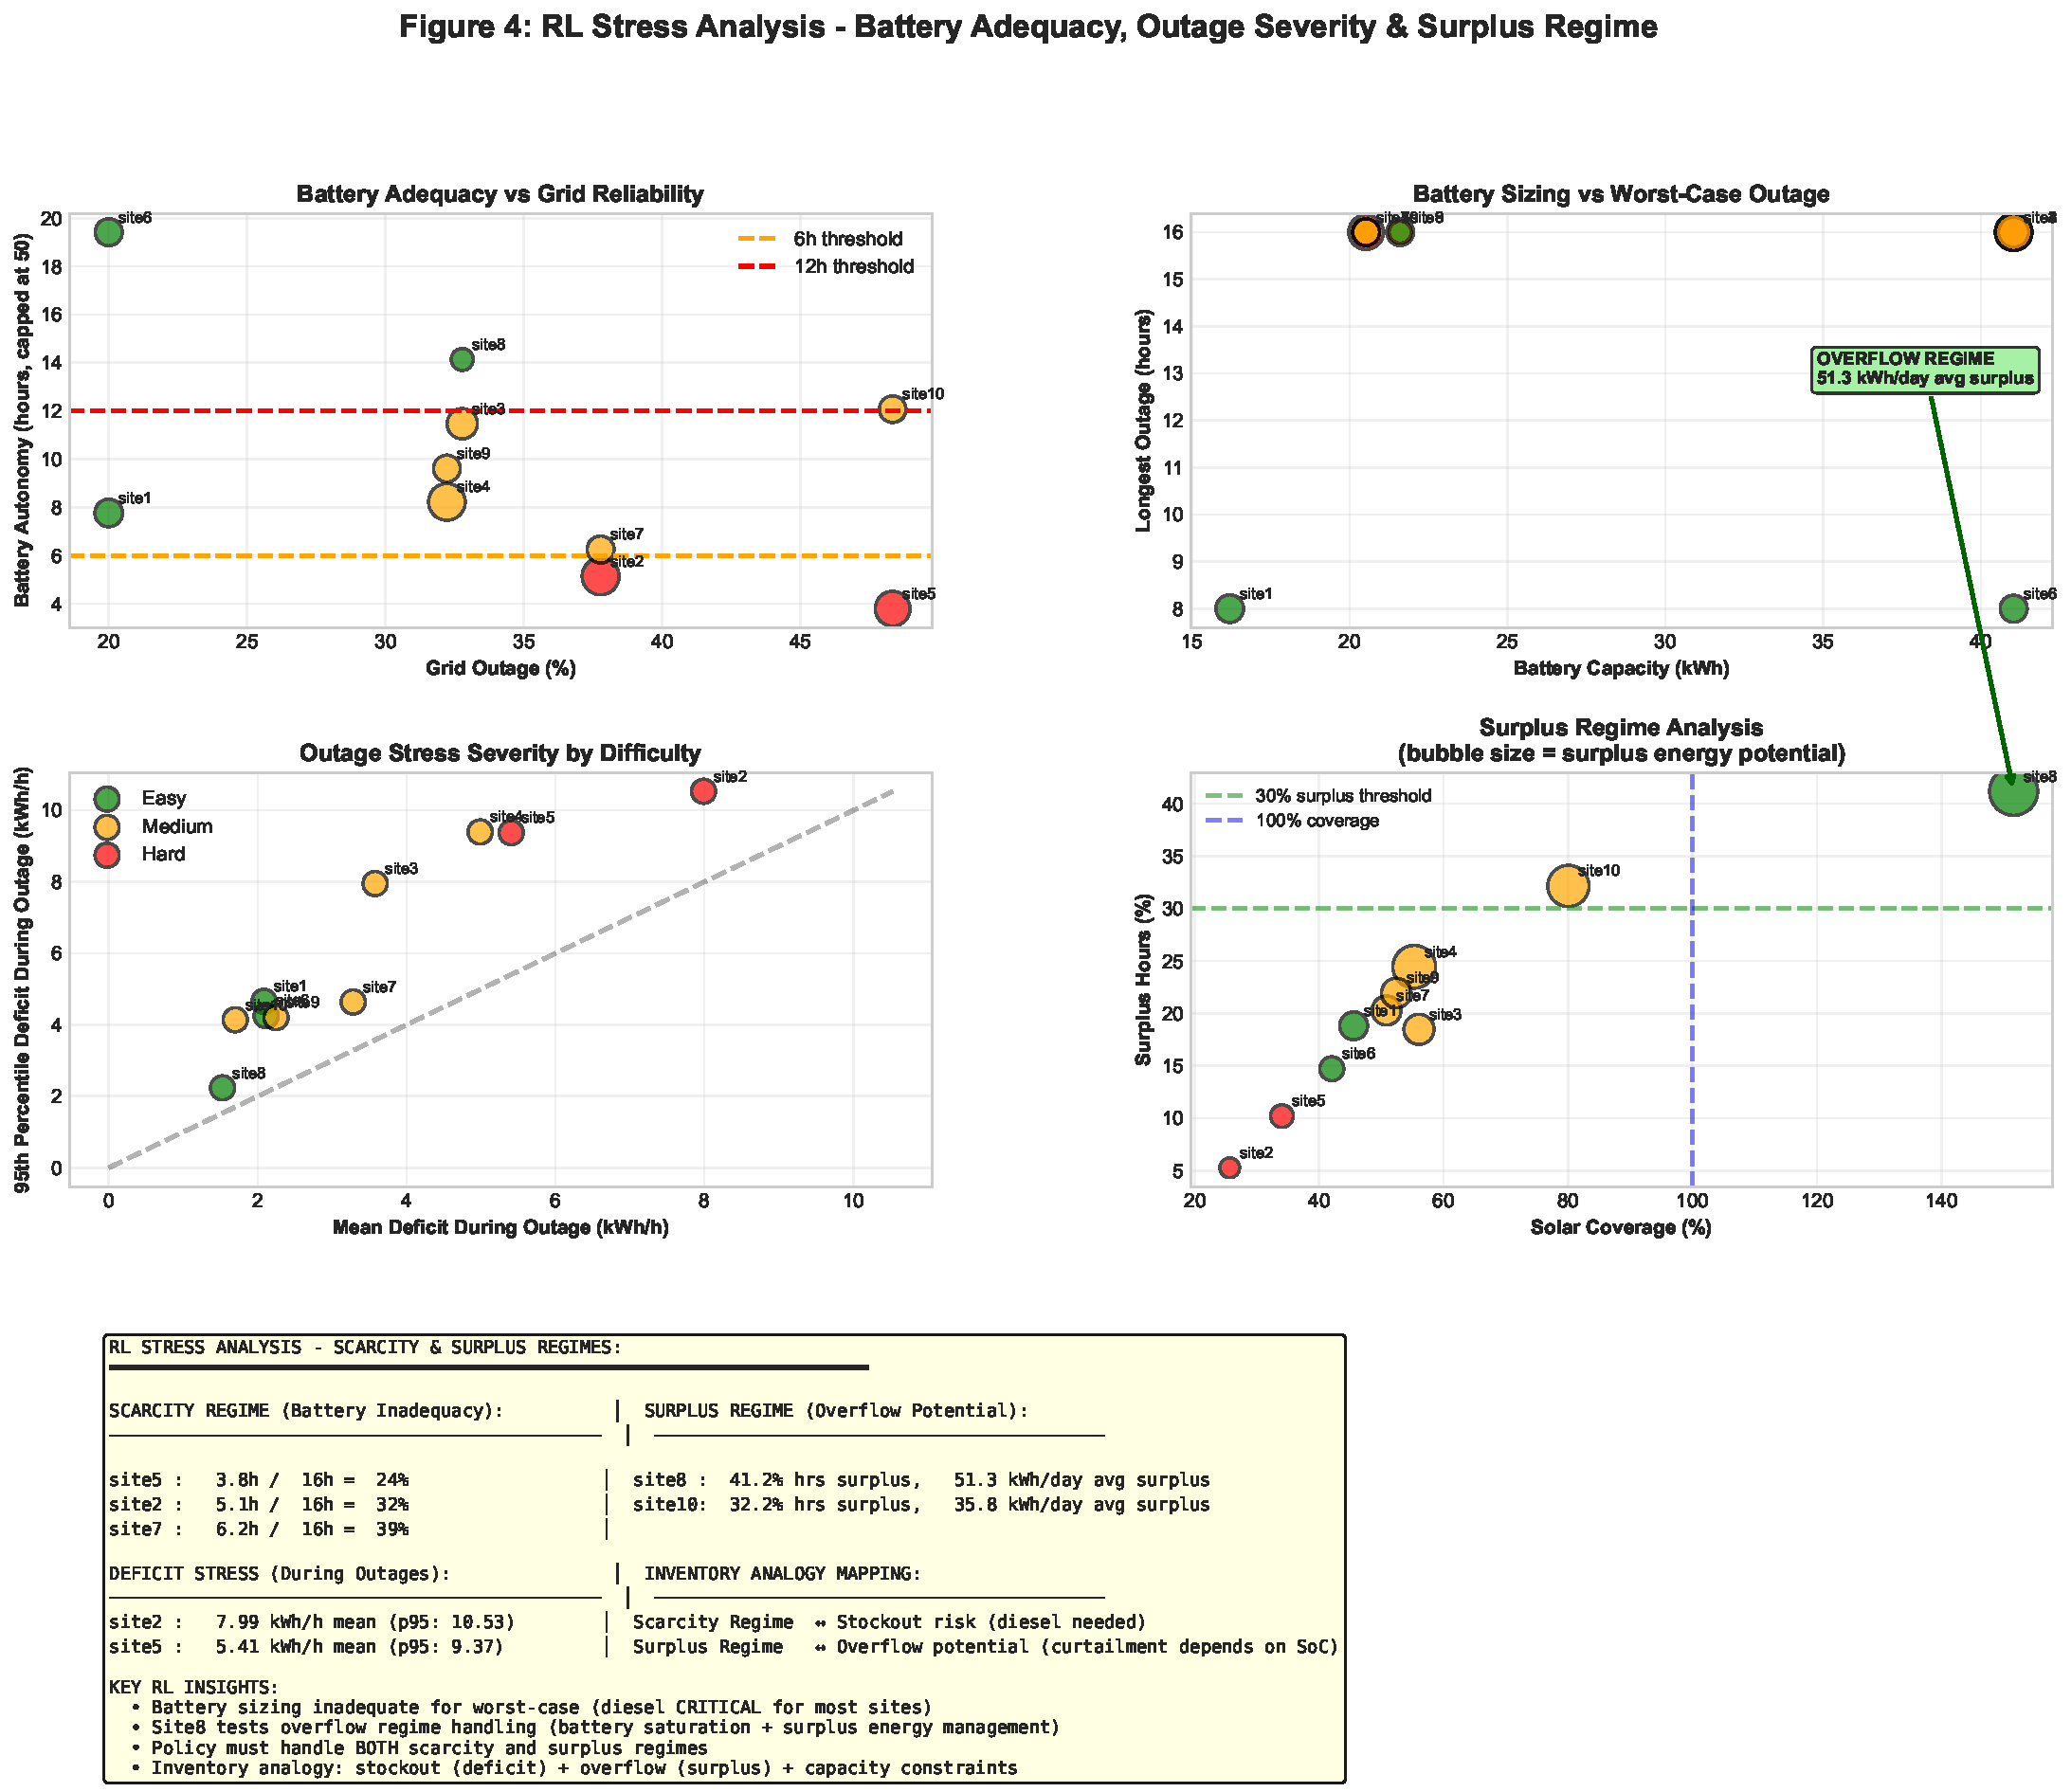
\includegraphics[width=\textwidth, clip=true]{images/fig4_rl_stress_analysis}
\caption{RL stress analysis across all ten sites.
\textit{Top-left:} battery autonomy (hours) vs.\ grid outage rate; sites
below the 6\,h threshold (orange dashed) cannot bridge a typical outage on
battery alone.  Sites~2 and~5 fall well below this line.
\textit{Top-right:} battery capacity vs.\ longest observed outage; most sites
face worst-case outages of 16\,h with batteries sized for far less.
\textit{Bottom-left:} mean vs.\ 95th-percentile deficit during outages;
sites~2 and~5 (red) show the highest deficit stress.
\textit{Bottom-right:} surplus hours vs.\ solar coverage; site~8 is in the
overflow regime with 41\% surplus hours and 51\,kWh/day average surplus.
The summary panel confirms the scarcity--surplus split: sites~2 and~5 are
battery-inadequate (inventory-critical), while site~8 and partially site~10
face overflow potential.}
\label{fig:rl_stress}
\end{figure}

Figure~\ref{fig:net_load_cdf} shows the net load
CDF for all sites; the Hard sites (site~2 and site~5, red) have right-shifted
distributions, confirming sustained positive net load and high reliance on
supplementary energy sources.

\textbf{Surplus regime.}
At the other extreme, site~8 is clearly solar-surplus, with solar coverage
of 151.6\% and net load negative for 41\% of hours (average surplus
51\,kWh/day).  Solar generation peaks at 10.5\,kWh/h near 10:00 while
load holds steady near 2\,kWh/h, saturating the 21.6\,kWh battery on
most days.  Here the main challenge is not avoiding shortage but handling
battery saturation and curtailment.  Site~8 behaves qualitatively
differently from the scarcity-dominated sites; its detailed profile is
in Appendix~\ref{app:site_profiles}.

\begin{figure}[htbp]
\centering
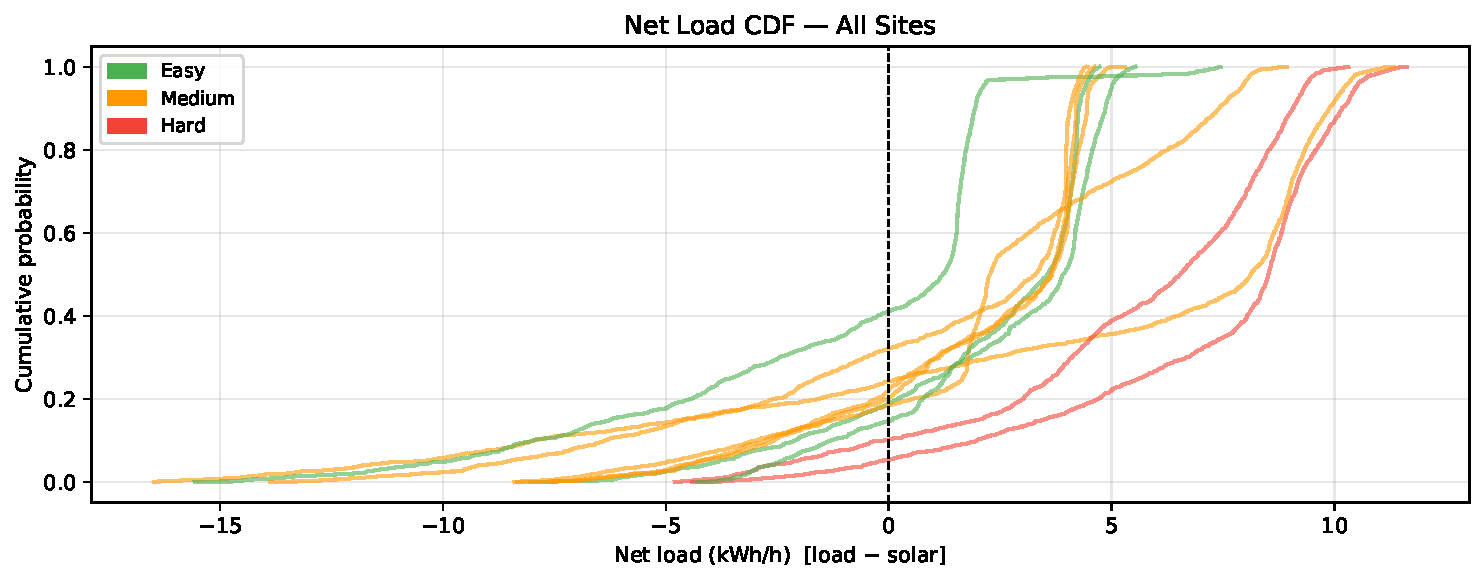
\includegraphics[width=0.85\textwidth, clip=true]{images/fig_net_load_cdf}
\caption{Cumulative distribution of net load across all sites.  The dashed
vertical line at zero separates solar-deficit hours (right) from solar-surplus
hours (left).  Hard sites (red) are entirely in deficit; site~8 (green) crosses
zero near $p = 0.6$, confirming majority solar surplus.}
\label{fig:net_load_cdf}
\end{figure}

This regime split is important for the experimental design.  Easy and
surplus-regime sites are useful robustness checks but offer limited
discriminatory power where operating conditions are mild.
The scarcity-regime sites --- primarily site~2, site~5, and site~10 under
adverse logistics conditions --- are structurally where inventory-aware
control is most likely to reveal a measurable advantage.

\begin{quote}
\textbf{Note on site terminology used elsewhere in this thesis.} This
scarcity-regime grouping (site~2, site~5, site~10) and the Hard/Medium/Easy
difficulty classification of Section~\ref{sec:site_classification} below
are both derived from the EDA in this chapter. A separate, differently
selected three-site subset (site~2, site~5, site~7) is used in
Chapter~\ref{chap:results} for finer-grained sensitivity analyses; that
subset was chosen to provide diverse operating characteristics (load,
solar generation and outage behaviour) for the detailed sensitivity
analyses, rather than to represent the scarcity-based difficulty ranking
introduced in this chapter. The scarcity-regime classification introduced
here is therefore used for exploratory data analysis, whereas the
site~2/site~5/site~7 subset supports the controlled experimental
comparisons described in Chapters~\ref{chap:methodology}
and~\ref{chap:results}.
\end{quote}


% ============================================================
\section{Representative Site Profile}
\label{sec:site_profiles}
% ============================================================

To make the stress analysis concrete, Figure~\ref{fig:site5_analysis}
presents the enhanced profile for site~5 --- the most operationally
demanding site in the dataset and the primary test case for
inventory-aware control.  Profiles for all ten sites are provided in
Appendix~\ref{app:site_profiles}.

Site~5 combines high outage frequency (52 events over 60 days, the
highest in the dataset), low solar coverage (34\%), and a small battery
(20.5\,kWh, autonomy 3.8\,h).  The battery covers only 24\% of the
longest observed 16-hour outage.  Four outage events exceed the 12-hour
threshold.  Outage-conditioned mean deficit is 5.41\,kWh/h (95th
percentile 9.37\,kWh/h).  Under these conditions any policy that
underestimates diesel consumption risk faces repeated unserved load
events.
 This site therefore provides one of the most discriminating test
cases for comparing inventory-aware and inventory-blind control.

\begin{figure}[htbp]
\centering
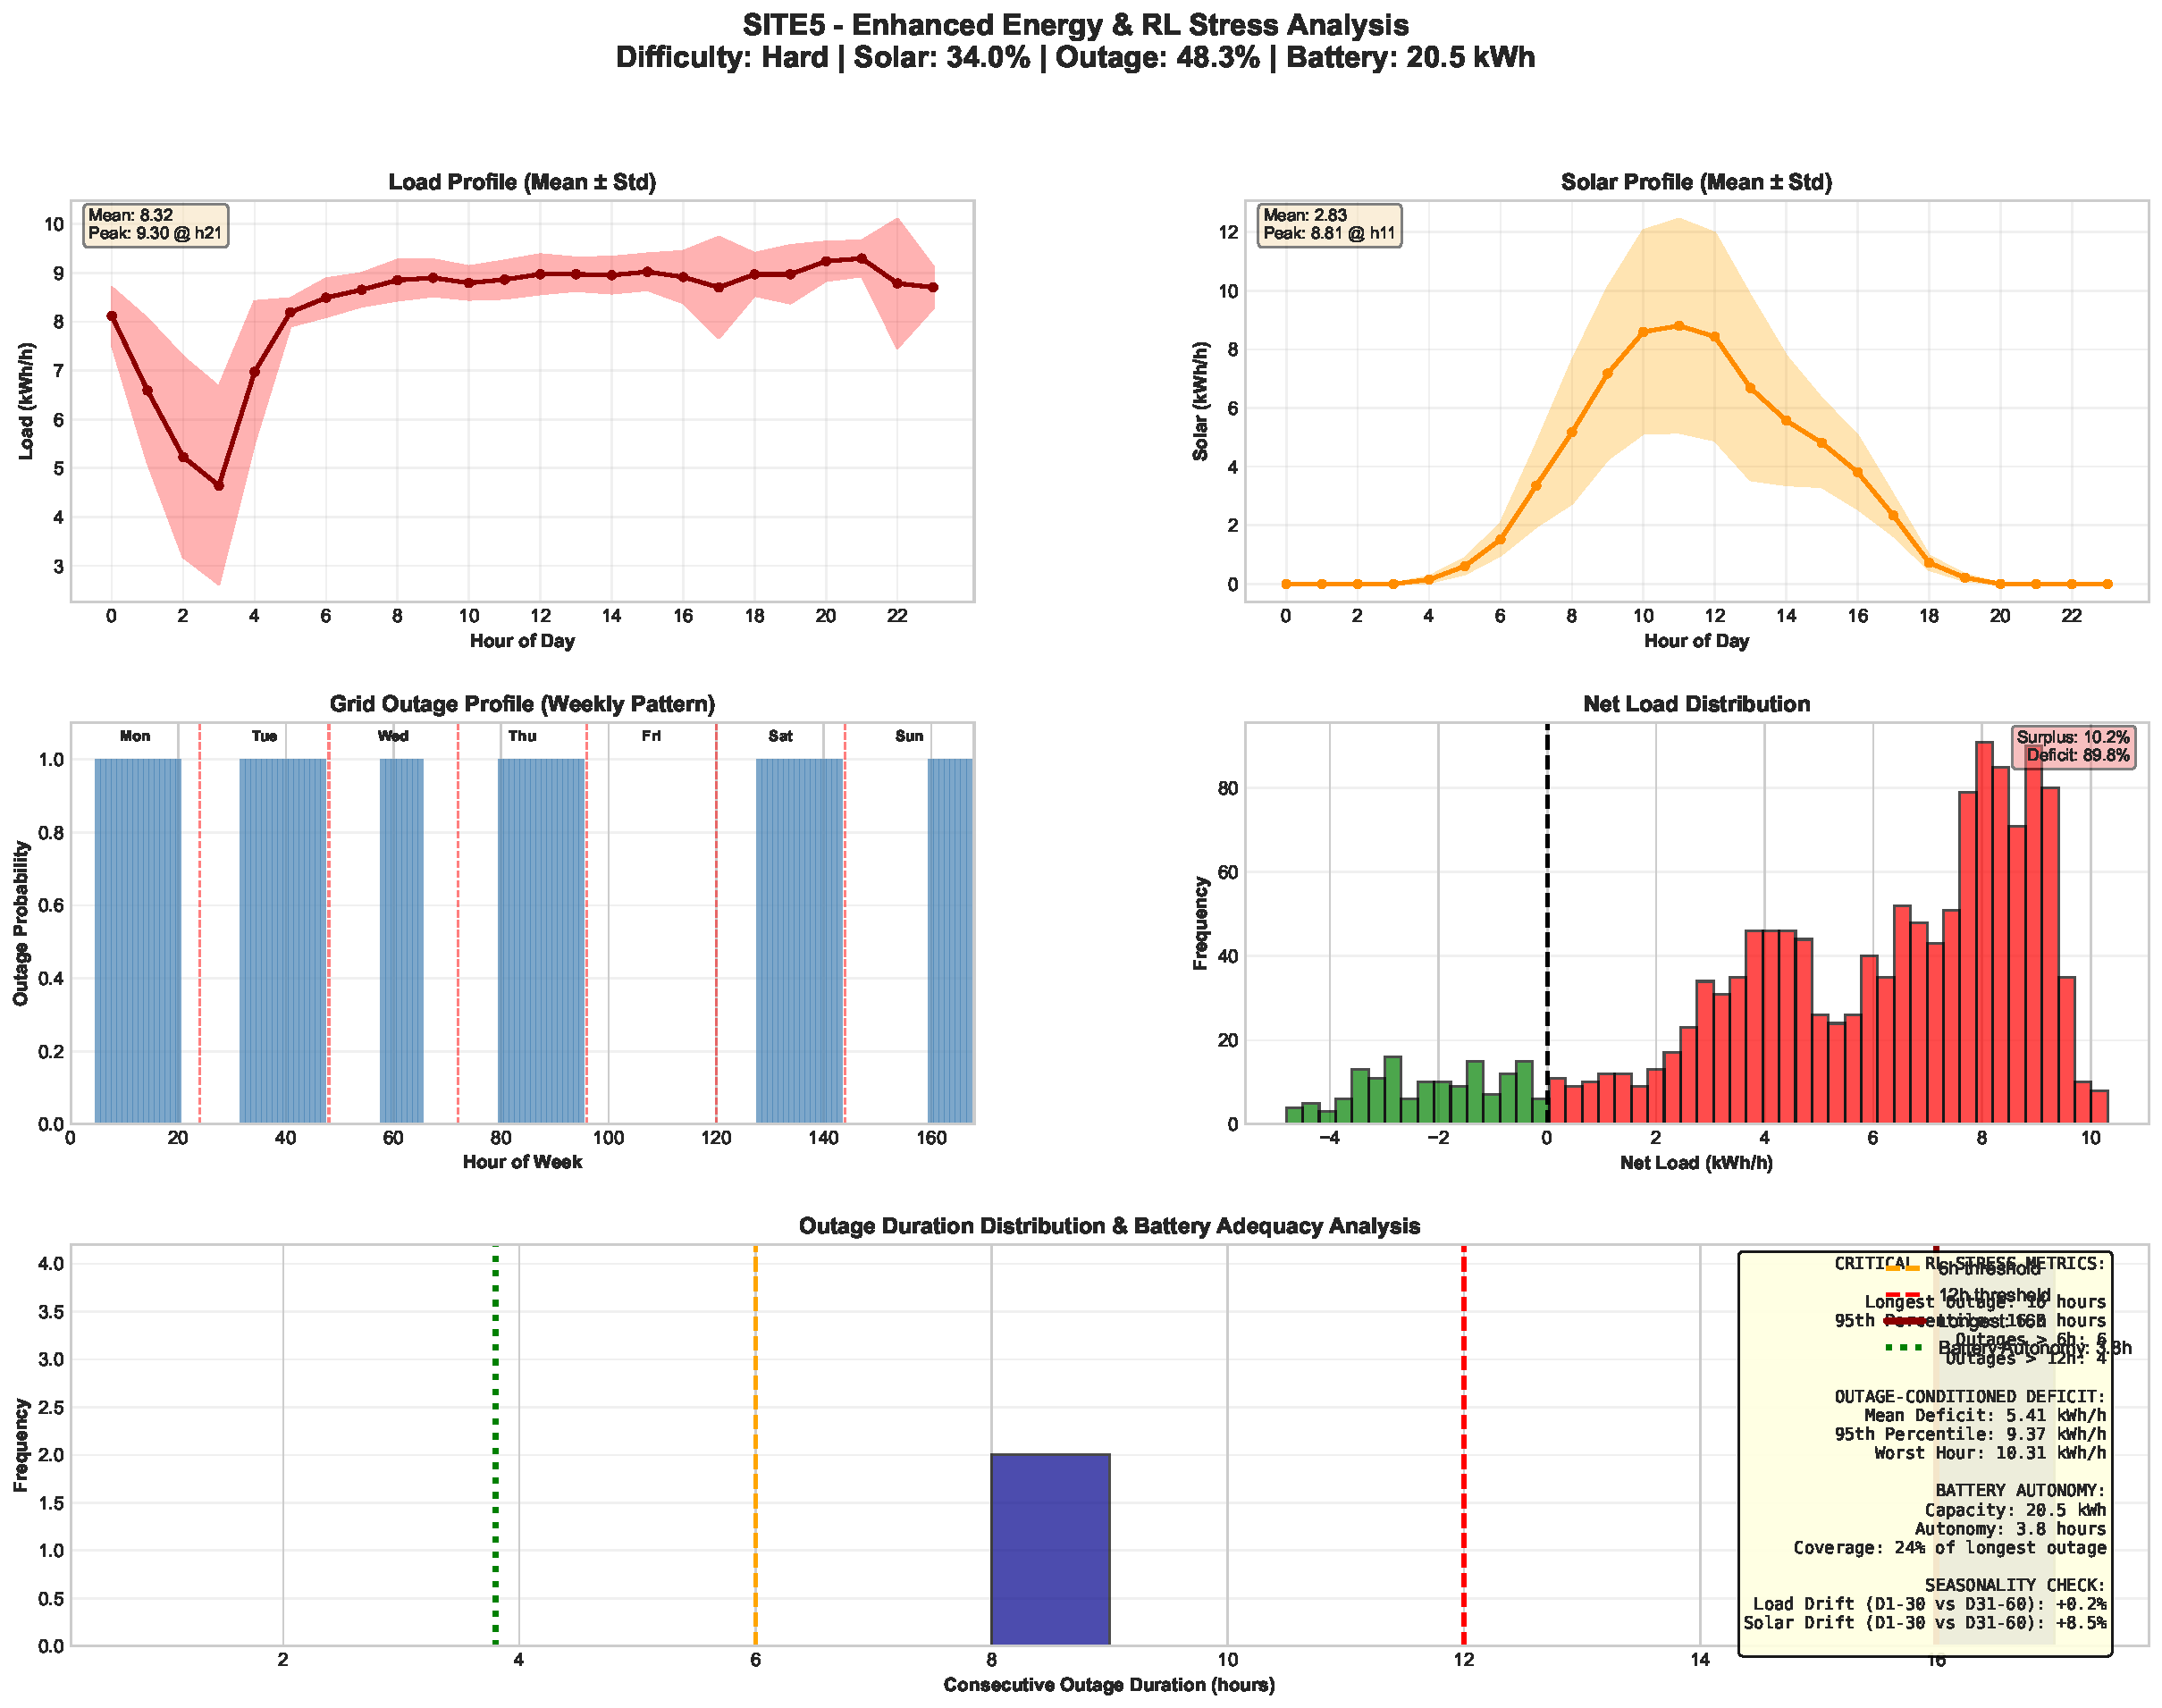
\includegraphics[width=\textwidth, clip=true]{images/site5_enhanced_analysis}
\caption{Enhanced stress analysis for site~5 (Hard).
Battery autonomy of 3.8\,h covers only 24\% of the longest outage.
52 outage events over 60 days --- the highest frequency in the dataset.
Four events exceed the 12-hour threshold (red dashed line).
Outage-conditioned 95th-percentile deficit is 9.37\,kWh/h.}
\label{fig:site5_analysis}
\end{figure}


% ============================================================
\section{Site Difficulty Classification}
\label{sec:site_classification}
% ============================================================

To organise the experiments, sites are grouped into difficulty classes using a
composite score combining grid outage frequency, solar coverage, and mean net
load.  Sites scoring 4 are classified Hard; 2 Medium; 1 Easy.
Table~\ref{tab:difficulty} shows the classification.

\begin{table}[htb]
\centering
\small
\caption{Site difficulty classification and primary challenge.  Constrained
sites (frequent outages, low solar, inadequate battery autonomy) receive
focused statistical analysis in Chapter~\ref{chap:results}.}
\label{tab:difficulty}
\begin{tabular}{p{3.8cm}p{1.5cm}p{1.5cm}p{5.0cm}}
\toprule
\textbf{Site(s)} & \textbf{Class} & \textbf{Outage (\%)} & \textbf{Primary challenge} \\
\midrule
site2, site5                       & Hard   & 38--48 & High load, low solar, frequent outages;
                                                        battery autonomy inadequate for longest outages \\
site3, site4, site7, site9, site10 & Medium & 33--48 & Moderate load-solar balance; grid
                                                        reliability moderate \\
site1, site6, site8                & Easy   & 20--33 & Adequate solar or high grid availability;
                                                        outage stress low \\
\bottomrule
\end{tabular}
\end{table}

\begin{quote}
\textbf{Note on site~10.}
Site~10 is classified Medium by composite score (solar coverage 80\%, but
outage frequency 51.7\%).  Its battery autonomy of 12.1\,h covers only
75\% of the longest observed 16-hour outage, and four outage events exceed
the 12-hour threshold.  Under adverse logistics conditions, site~10 is
structurally exposed to the same reliability risks as the Hard sites.
Results tables note this distinction where relevant.
\end{quote}

The classification is a practical organising tool, not a research outcome.
It separates sites where operating stress is structurally high
from those where conditions are comparatively mild.


% ============================================================
\section{Dataset Limitations}
\label{sec:dataset_limitations}
% ============================================================

The dataset is well suited to the present study, but three limitations must
be stated clearly.

\textbf{No diesel logistics records.}
The dataset provides load, solar, grid availability, and battery capacity, but
not diesel delivery events, lead times, or fuel replenishment logs.  The
delivery-pipeline component of the simulator is therefore synthetic.  This
is the sole component of the simulation not grounded in the ITU data, and
is clearly documented as such in Chapter~\ref{chap:methodology}.

\textbf{Limited time horizon.}
Each site contains 60 days of observations, covering a single operating
season.  Solar generation patterns and outage frequencies may differ in other
seasons; results should be interpreted as representative of the recorded
conditions rather than year-round operation.

\textbf{Assumed tank capacity.}
Absolute diesel tank capacity is not provided.  The assumption
$C^{\Tank} = 72\bar{D}$ gives physically plausible values (approximately
three days of full-load backup across all sites), but real tank sizes may
differ.  Sensitivity to this assumption is partially captured by randomising
initial inventory over $[0.3,\,0.9]\,C^{\Tank}$ during evaluation.


% ============================================================
\section{Chapter Summary}
\label{sec:dataset_summary}
% ============================================================

This chapter established the empirical foundation of the study.  The
ITU/Zindi dataset provides ten heterogeneous tower sites with hourly load,
solar, and grid traces that are replayed directly in the simulator.
Preprocessing produces clean site-level time series with consistent indexing,
derived net load, and a principled train/test split.  Exploratory analysis
shows that the sites span both scarcity-dominated and surplus-dominated
regimes, with large differences in outage severity, battery adequacy, and
renewable coverage.  These characteristics justify the multi-site evaluation
design used in the remainder of the thesis and explain why inventory-aware
control is most likely to show a measurable advantage in the most constrained
sites.